\section[Effects on downstream analysis]{Effects of additional somatic variants on downstream analysis}
\label{variantcalling-sec:downstream}

The ability to find additional shared variants has significant impact on our understanding of cancer evolution and the timing of initiation and metastatic seeding. Recent work has shown, that similar to the well known genetic heterogeneity, there is heterogeneity when it comes to the timing of metastatic seeding. While traditionally it was thought that tumours only metastasise after they reach a certain size, to escape the restrictions of the niche, like reduced nutrition, recent publications showed, there is also very early metastatic seeding \cite{Hu2019}. 
But all methods analysing heterogeneity, evolutionary timing and history are fully reliant on the somatic variants found in the data. Therefore, if we improve the input provided to these analysis methods, we can expect a clearer and possibly more granular result.

The following section will quantify the effect of additionally found variants on phylogenetic reconstruction and clonal decomposition, which use somatic variants as input.


\subsection[Phylogenetic reconstruction]{Phylogenetic reconstruction}
\label{variantcalling-sec:phylo}
As this work is not about the advantages and shortcomings of different phylogenetic reconstruction tools, we have not performed a comprehensive comparison of these tools, but rather focused on the results of using additional variants.  For this reason, we chose to use neighbour joining (NJ) \cite{Saitou1987}, because it is fast, readily available in most phylogenetic reconstruction tool kits and if the input distance is correct, the output will be correct. And even, if the distance is not 100\% correct, if the distance is ``nearly additive`` and the input distances are not far off from the real distance, the tree topology will still be reconstructed correctly \cite{Mihaescu2007}. Lastly, in contrast to many other methods like UPGMA and WPGMA \cite{Sokal1958}, NJ does not assume an equal mutation rate of each sample, because we know, that the molecular clock hypothesis \cite{Zuckerkandl1962} is not valid for different lineages of cancers \cite{Shibata2010}.

The only thing that NJ requires as an input is a distance matrix of all samples, so the next step was the selection of the right distance metric. While there are many distance measures for DNA sequences, which allow accounting for different probabilities of transitions and transversions as well as uneven base composition, models like F81 \cite{Felsenstein1981} or HKY85 \cite{Hasegawa1985} are only really designed for germline mutations and are not easily applicable for subclonal somatic mutations, which is why we decided to first transform the variants present in all samples into a binary occurrence vector and then calculating the Hamming distance \cite{Hamming1950} between all samples. This generates a maximum parsimony approach and the branch length of the trees will be directly translatable to the amount of variants which are different between samples. 

\autoref{fig:ca9phylo} shows both the reconstructed phylogenies of the autopsy samples of the late stage melanoma patient ``CA-F`` from the manuscript (\autoref{ch:appendixManuscript}, \autoref{A:tab:S1}), using the variants found with the default tumour-normal method on the left and our improved joint method on the right. The exact same reconstruction methodology was used otherwise, such that only the different inputs lead to the final difference.

\begin{figure}[ht]
\centering
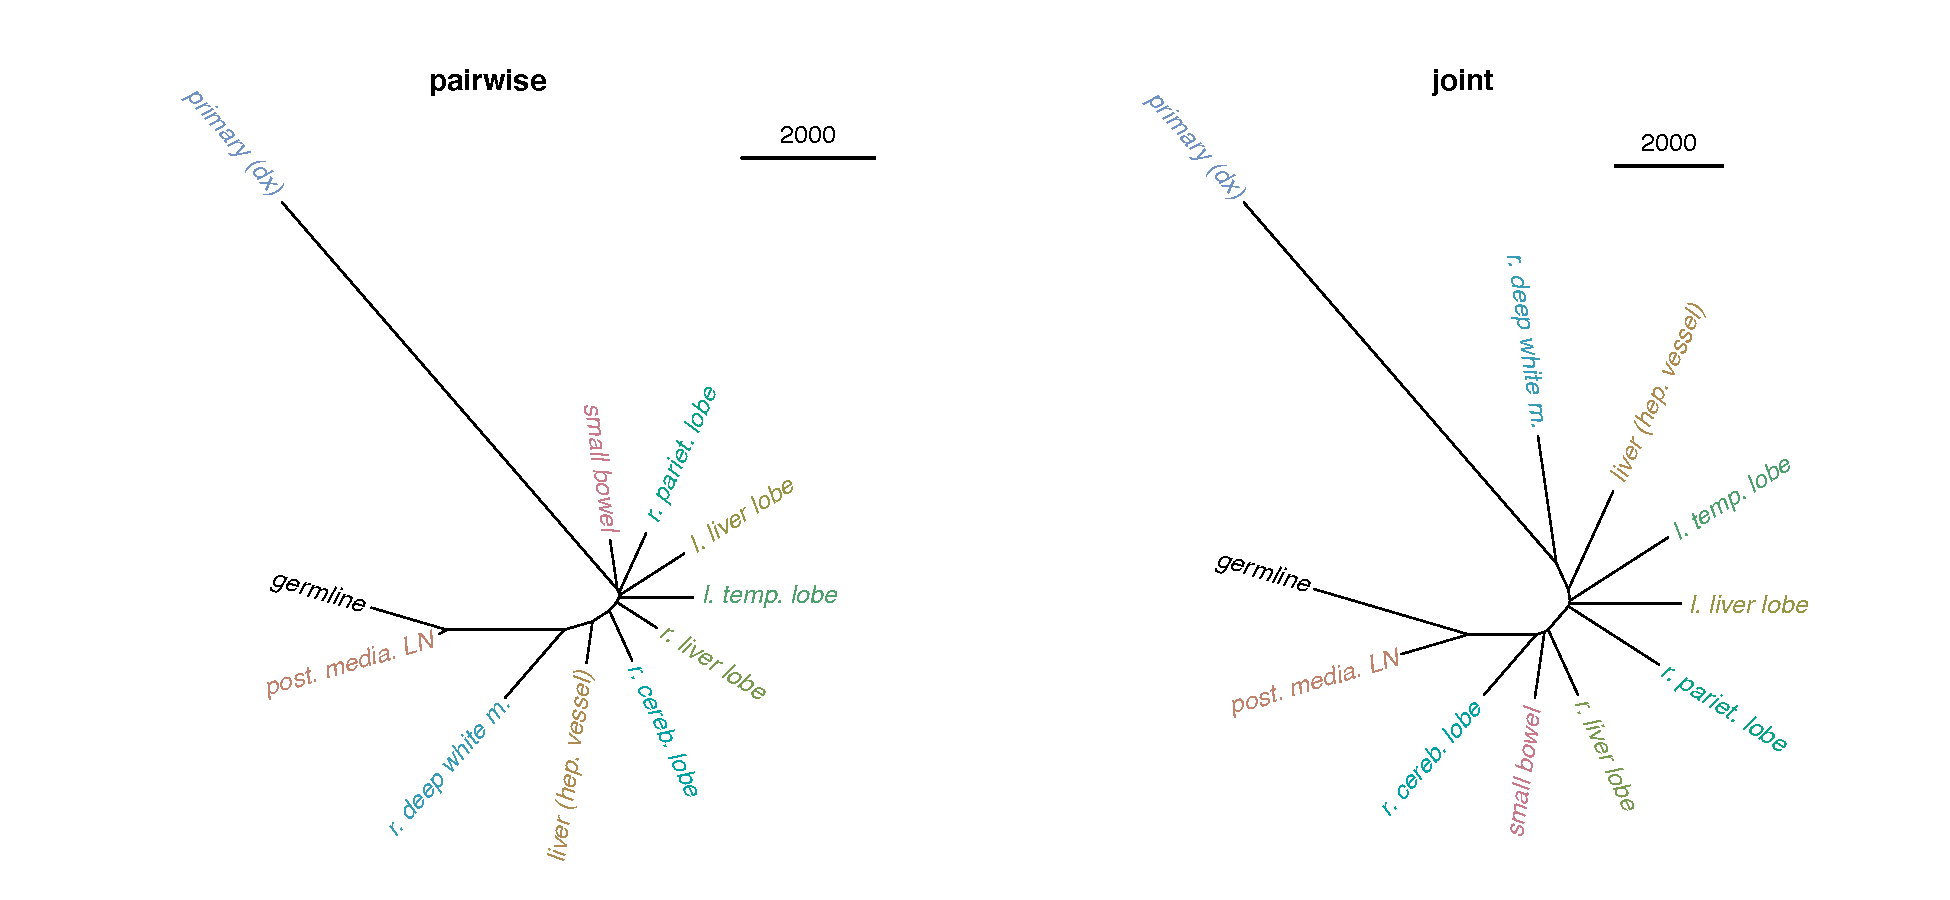
\includegraphics[width=.99\linewidth]{Figures/jointVariantCalling/phyloCA9.pdf}
\caption[Reconstructed phylogenies of joint samples]{Reconstructed phylogenies of a patient with multiple spatially distinct samples; Neighbour joining on Hamming distance on variant occurrence vector. Tip labels describe the location of the sample in the patient. Trees are shown as unrooted with germline as fixated origin point; black line ruler shows the length of an edge with 2000 mutations}\label{fig:ca9phylo}
\end{figure}

\todo[inline, color=green]{Maybe adjust the font size in the trees to make it more readable}

There are several obvious changes, first in the longer edge connecting the germline to all other samples, which we consider as the state of no somatic variants. This shows that there are many more shared mutations in all samples, than what would have been anticipated with the default method, which corresponds to an overestimation of the heterogeneity of the samples. As the accumulation of somatic variants is still used as a proxy for timing and cell divisions, when assuming a high mutation rate for lung cancer ($5.3 \cdot 10^{-8}$ from \citeauthor*{Werner2020} \cite{Werner2020}) this difference of $\approx 36000$ variants is equivalent to $\approx 2000$ cell divisions. While the cell doubling rate of lung cancers is highly dependent on the type \cite{Arai1994}, this change makes a substantial difference when assessing the timing of the tumour initiation and further evolution. 

Secondly, there have been topological changes, which generate a longer bifuricating edge between the olive coloured ``r. liver lobe`` and the ``r. pariet. lobe`` showing a bottle neck in cancer evolution, which fits very well with the clinical history, where the patient lived with stable disease for almost ten years, before progressing and dying. The extreme distance of the primary/diagnostic sample from the rest of the samples could be either a difference in sequencing quality, or due to the exposure to FFPE for the ten years between tumour diagnosis and death. However, as this feature is preserved between both the joint and the pairwise analysis, it does not appear to be an effect of our new method.

\begin{figure}[ht]
\centering
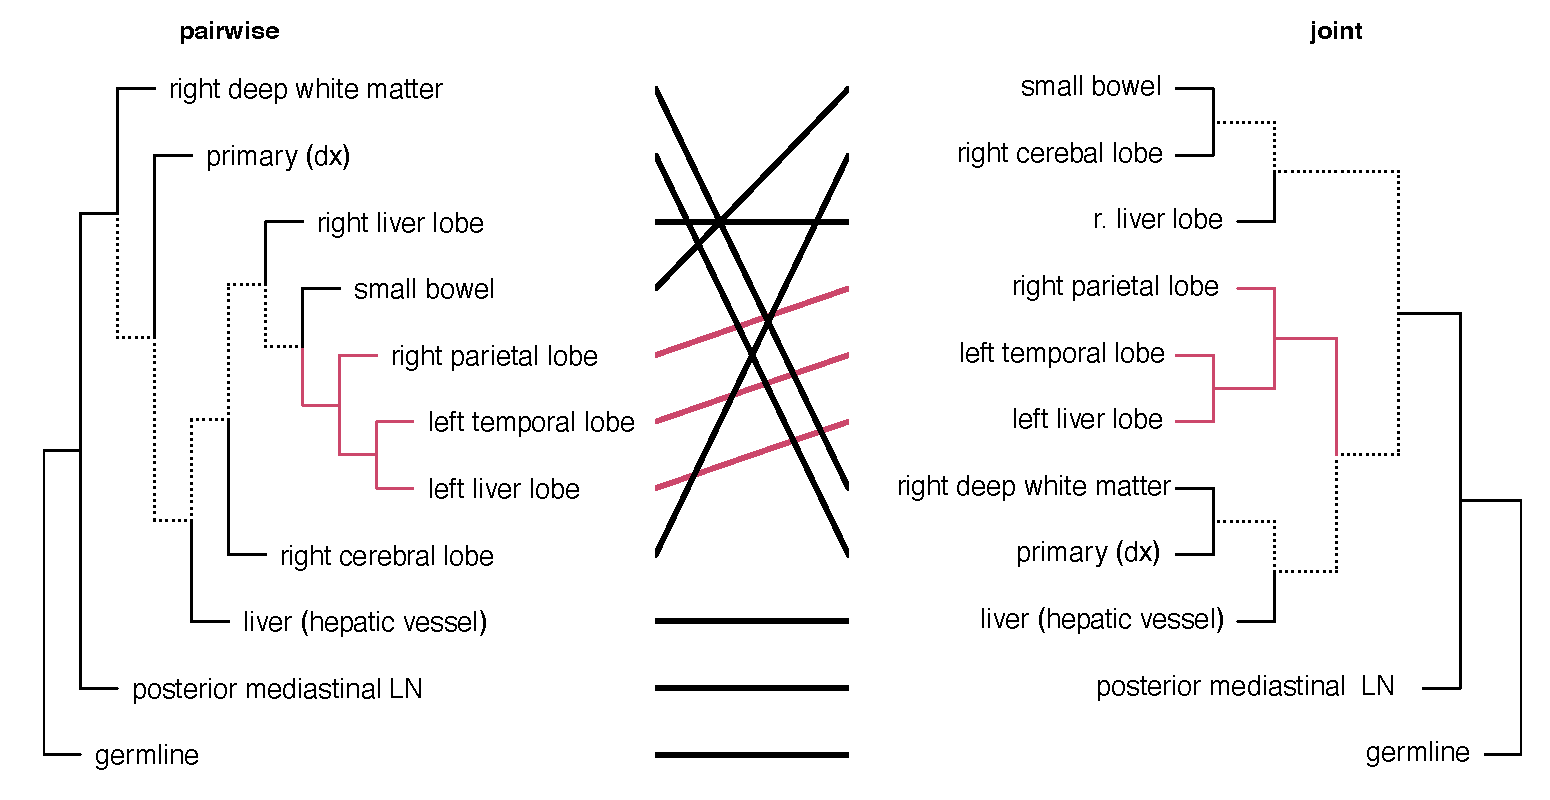
\includegraphics[width=.99\linewidth]{Figures/jointVariantCalling/tanglePhyloCA9.pdf}
\caption[Tanglegram of the reconstructed phylogenies]{Side by side view of the reconstructed trees from \autoref{fig:ca9phylo}; internal edges, which are distinct between trees are shown as dotted lines; common subtree is shown in red  Tree labels have been sorted to minimise distance between labels; Visualisation generated with dendextend \cite{Galili2015}}\label{fig:tanglePhyloCA9}
\end{figure}
\todo[inline, color=green]{maybe increase the line width of the edges}

\autoref{fig:tanglePhyloCA9} shows a topology focused view of the two trees, which highlights the breaks which are needed to morph one tree into the other with dotted edges \cite{Vienne2018}. The common subtrees are coloured the same on both sides and connecting lines show identical labels. This format shows that while the trees look quite similar at first glance, they show vastly different topologies.


One example of this is ``small bowel`` which was connected to the red common subtree, but is now much closer to the ``r. cereb. lobe`` and forms a parallel clade with the ``r.liver lobe``. In general, where the pairwise tree shows a very linear topology, which leaves only branching out of the main with no disjunct subclades, which are clearly present in the joint reconstruction.  (\autoref{fig:tanglePhyloCA9}).


\section[Longitudinal analysis]{Longitudinal analysis}
\label{variantcalling-sec:longitudinal}

The initial motivation for the development of our workflows was the analysis of multi-region, or spatial, samples from the same patient coming from the CASCADE rapid autopsy program. However, we were very interested on applying the methods on longitudinal samples from patients, for example, for the joint analysis of diagnostic and relapse sample, or even the repeated testing of ctDNA are quite worth thinking about. In this part, we present work using the published workflows on a longitudinal dataset, which highlights the flexibility and widespread usability of the new methods.

In addition to their autopsy which resected nine distinct metastatic sites (\autoref{fig:CA-Fschematic}), Patient ``CA-F`` also had three longitudinal blood samples taken, from which ctDNA was extracted and WES performed. These blood samples were taken as non-invasive surveillance seven, five and two months before the death of the patient (\autoref{fig:CA-Ftimeline}). In a study of late stage melanoma patients, \Citeauthor{Tan2019} identified ctDNA sequencing as a way to stratify patients into high and low risk of relapse and therefore inform adjuvant therapy \cite{Tan2019}. This makes patient ``CA-F`` a very good test dataset to showcase the improvement with joint variant calling. Similar to the spatially related samples, the joint analysis can improve the performance, which then in turn enable the detection of lower allele frequency variants, either through lower tumour burden or through the limited availability of DNA fragments from brain lesions due to the blood brain barrier \cite{2014}.

\begin{figure}[ht]
\centering
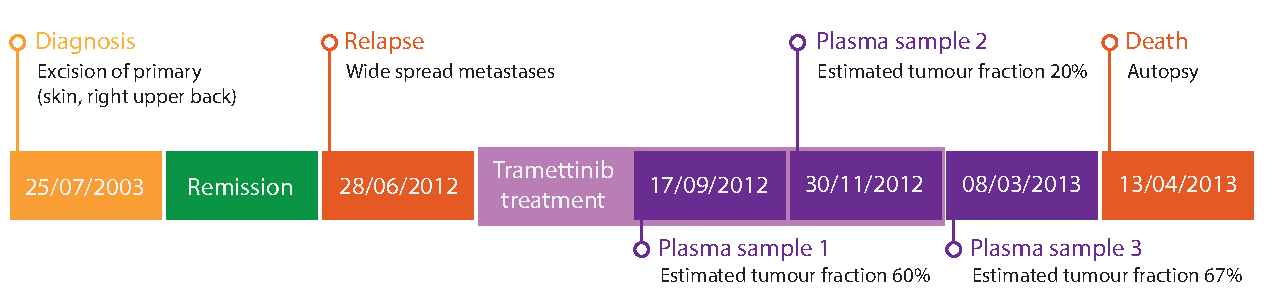
\includegraphics[width=.99\linewidth]{Figures/jointVariantCalling/CA-F_timeline.pdf}
\caption[Timeline from diagnosis till death for patient CA-F]{Timeline from diagnosis till death for patient CA-F: 1.9mm melanoma removed after diagnosis \dateenglish\formatdate{25}{07}{2003} but with negative sentinel lymph node biopsy; \dateenglish\formatdate{28}{06}{2012}: PET scan and subsequent liver biopsy confirm relapse with wide spread metastases; trametinib treatment from Oct. 2012 till Jan. 2013 with minor response; blood plasma samples during treatment (1 and 2) as well as after progression (3); death and rapid autopsy of nine metastatic sites (\dateenglish\formatdate{13}{04}{2013}, \protect\autoref{fig:CA-Fschematic}); Tumour fraction in plasma samples was estimated via the original driver mutation (BRAF:K601E)}\label{fig:CA-Ftimeline}
\end{figure}


To show that even in longitudinal data, the joint analysis can boost the signal, we jointly variant called the diagnostic biopsy sample with the three ctDNA samples and compared them with the results from the pairwise analysis. On average, we found 2905 additional variants in each of the ctDNA samples, which is more than doubles the average number of variants found with the pairwise analysis (2414). Out of those, we found 534 variants in the ctDNA samples, which were found as a high confidence variant in the diagnostic sample, indicating that these findings are high quality calls. 

\begin{figure}[ht]
\centering
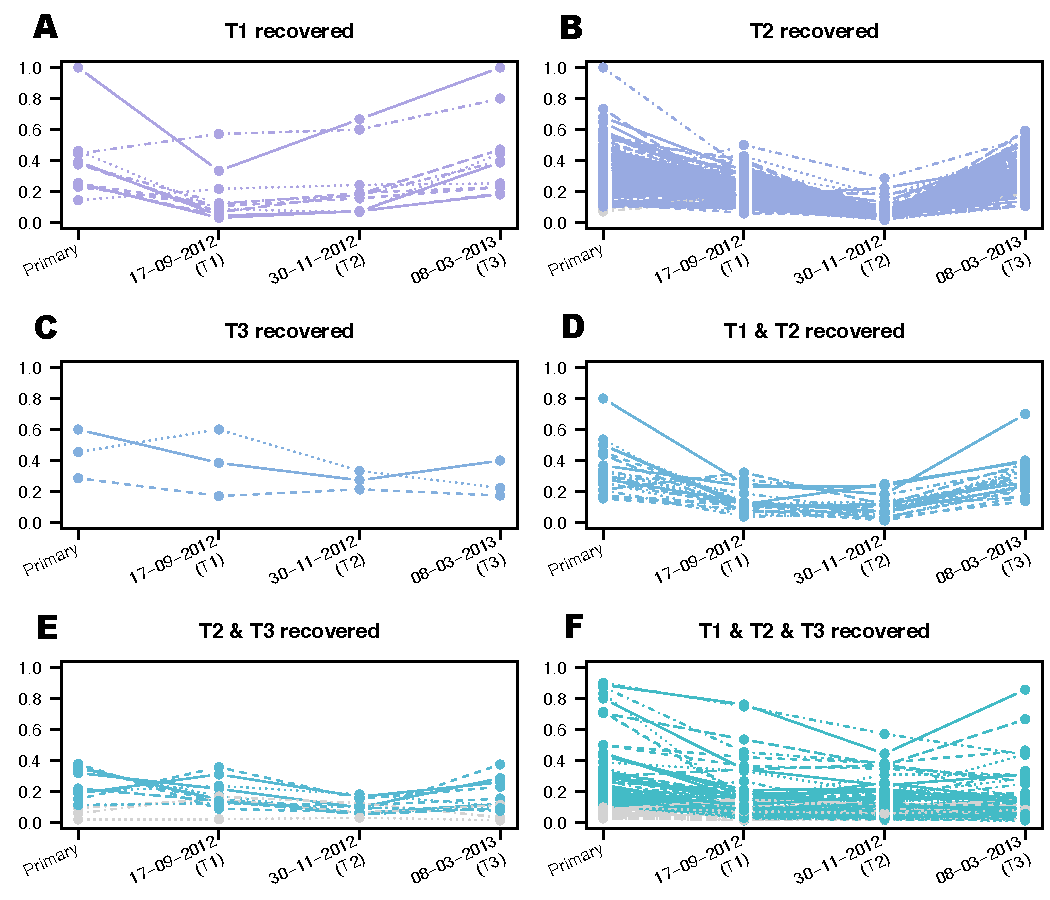
\includegraphics[width=.99\linewidth]{Figures/jointVariantCalling/longitudinalCA9ctDNAVafs.pdf}
\caption[Improved somatic variant calling in longitudinal data]{Improved somatic variant calling in longitudinal data: Variant allele frequency (VAF) of variants found additionally through joint variant calling which were found as high confidence variants in the primary sample; Variants with less than 0.1 VAF in the primary are coloured grey; ``T1 recovered`` shows variants, which were high confidence in all ctDNA samples but T1 and were only found through joint calling there; Axis label show the date of blood collection }\label{fig:longitudinalVAFsctDNA}
\end{figure}

Exactly like in the spatially different samples, in longitudinal data lower tumour purity samples benefit more from the joint analysis. We see that time point 2 (T2) has the highest amount of recovered variants (377) which are found as high confidence variants in both other time points (\autoref{fig:longitudinalVAFsctDNA} A vs. B vs. C) and T2 also has the lowest tumour purity in the cfDNA recorded (T1: 60\%; T2: 20\%; T3: 60\%) however, there are still 106 variants, which were not found in the ctDNA samples at all with the pairwise analysis at all, even though they were high confidence variants in the primary sample (\autoref{fig:longitudinalVAFsctDNA}F). These variants usually show a lower depth of coverage (dp) in the ctDNA samples, which may possibly indicate a problematic region in the genome, but rather than it not being called a variant, it is just a sign of incomplete data, which can be used with our joint approach. 

\begin{figure}[ht]
\centering
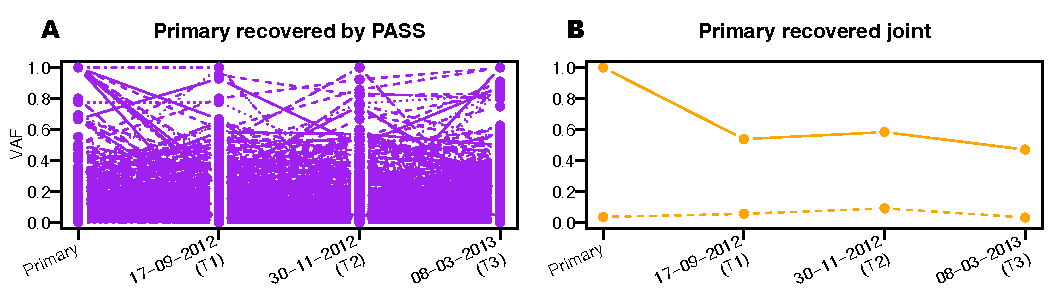
\includegraphics[width=.99\linewidth]{Figures/jointVariantCalling/longitudinalCA9primaryVafs.pdf}
\caption[Longitudinal data informs diagnostic variant calling]{Longitudinal data informs diagnostic variant calling: Vafs of variants additionally found through joint calling in the primary samples; Primary recovered by PASS shows variants which were high confidence in at least one ctDNA sample; Primary recovered joint shows variant which were low confidence in all samples in the pairwise analysis; Axis label show the date of blood collection}\label{fig:longitudinalVAFsprimary}
\end{figure}


Finally, we can also find 398 additional variants in the   primary sample. 398 were discarded due to missing data in the tissue sequencing, but could be found with a high confidence in the longitudinal data and two of the variants were included, as all 4 samples had this variant below the detection threshold (\autoref{fig:longitudinalVAFsprimary}). The missing depth in the primary also leads to the occasional very high allele frequency of the variant, as all available reads show the variant, but their numbers are below the threshold normal variant callers will report variants.

This shows that both spatially and longitudinal related samples should be analysed jointly, as it substantially increases the amount of true variants found, which as shown before, can have a large impact on downstream analysis of the samples.



\subsection[Clonal deconvolution]{Clonal deconvolution}
\label{variantcalling-sec:clonal}

On of the most important information derived from multiple related samples from the same patient is the clonal deconvolution, where subclonal reoccurring patterns of mutations (clones) are resolved both spatially and longitudinally. These reoccurring clones can be linked to either parallel evolution through positive selection pressure, like a targeted drug, or to the process of developing metastases where a piece of the cancer ``breaks`` off and grows at a different site.
In contrast to the lack of options for joint somatic variant calling, there is a plethora of algorithms and methods available for clonal deconvolution. Since 2015 PhyloWGS \cite{Deshwar2015}, Canopy \cite{Jiang2016}, CLOE \cite{Marass2016}, CloneFinder \cite{Miura2018}, MACHINA \cite{ElKebir2018} and MOBSTER \cite{Caravagna2020} were published, to name a few. Underlying all these models is a form of clustering variants with similar variant allele frequency together, to reduce the combinatorial space and enhance the confidence in the signal \cite{Tarabichi2021}. Due to the high number of tools, it is very challenging to select the right tool, especially since all of them have advantages and disadvantages \cite{Miura2020}. In this work we decided to use PhylogicNDT \cite{Leshchiner2018} as it has been shown to work well on clinical samples \cite{Gerstung2020} and does not have the restriction for the input to be from copy number neutral areas which many of the other tools have.


Both the variants found with the default pairwise as well as with the new joint workflows were annotated with their local allele specific copy number to form a MAF like file format which is required by PhylogicNDT. While PhylogicNDT allows the user to supply the cancer cell fraction for every variant, the program can also estimate them from the supplied allelic counts and the copy number. Local copynumber calls were derived from copy number segment calls made by sequenza by intersecting chromosomal location of each variant with the copy number segment containing the variants location. This requires multiple steps and the source code is shown in \autoref{lst-jvcAppendix:parseVcf} (parsing VCF), \autoref{lst-jvcAppendix:cnv} and \autoref{lst-jvcAppendix:convertMAF} (convert to MAF format). Variants which couldnt be annotated with copy number information, because their genomic location did not overlap with any called copy number segment, were discarded for this analysis.

\begin{figure}[ht]
\centering
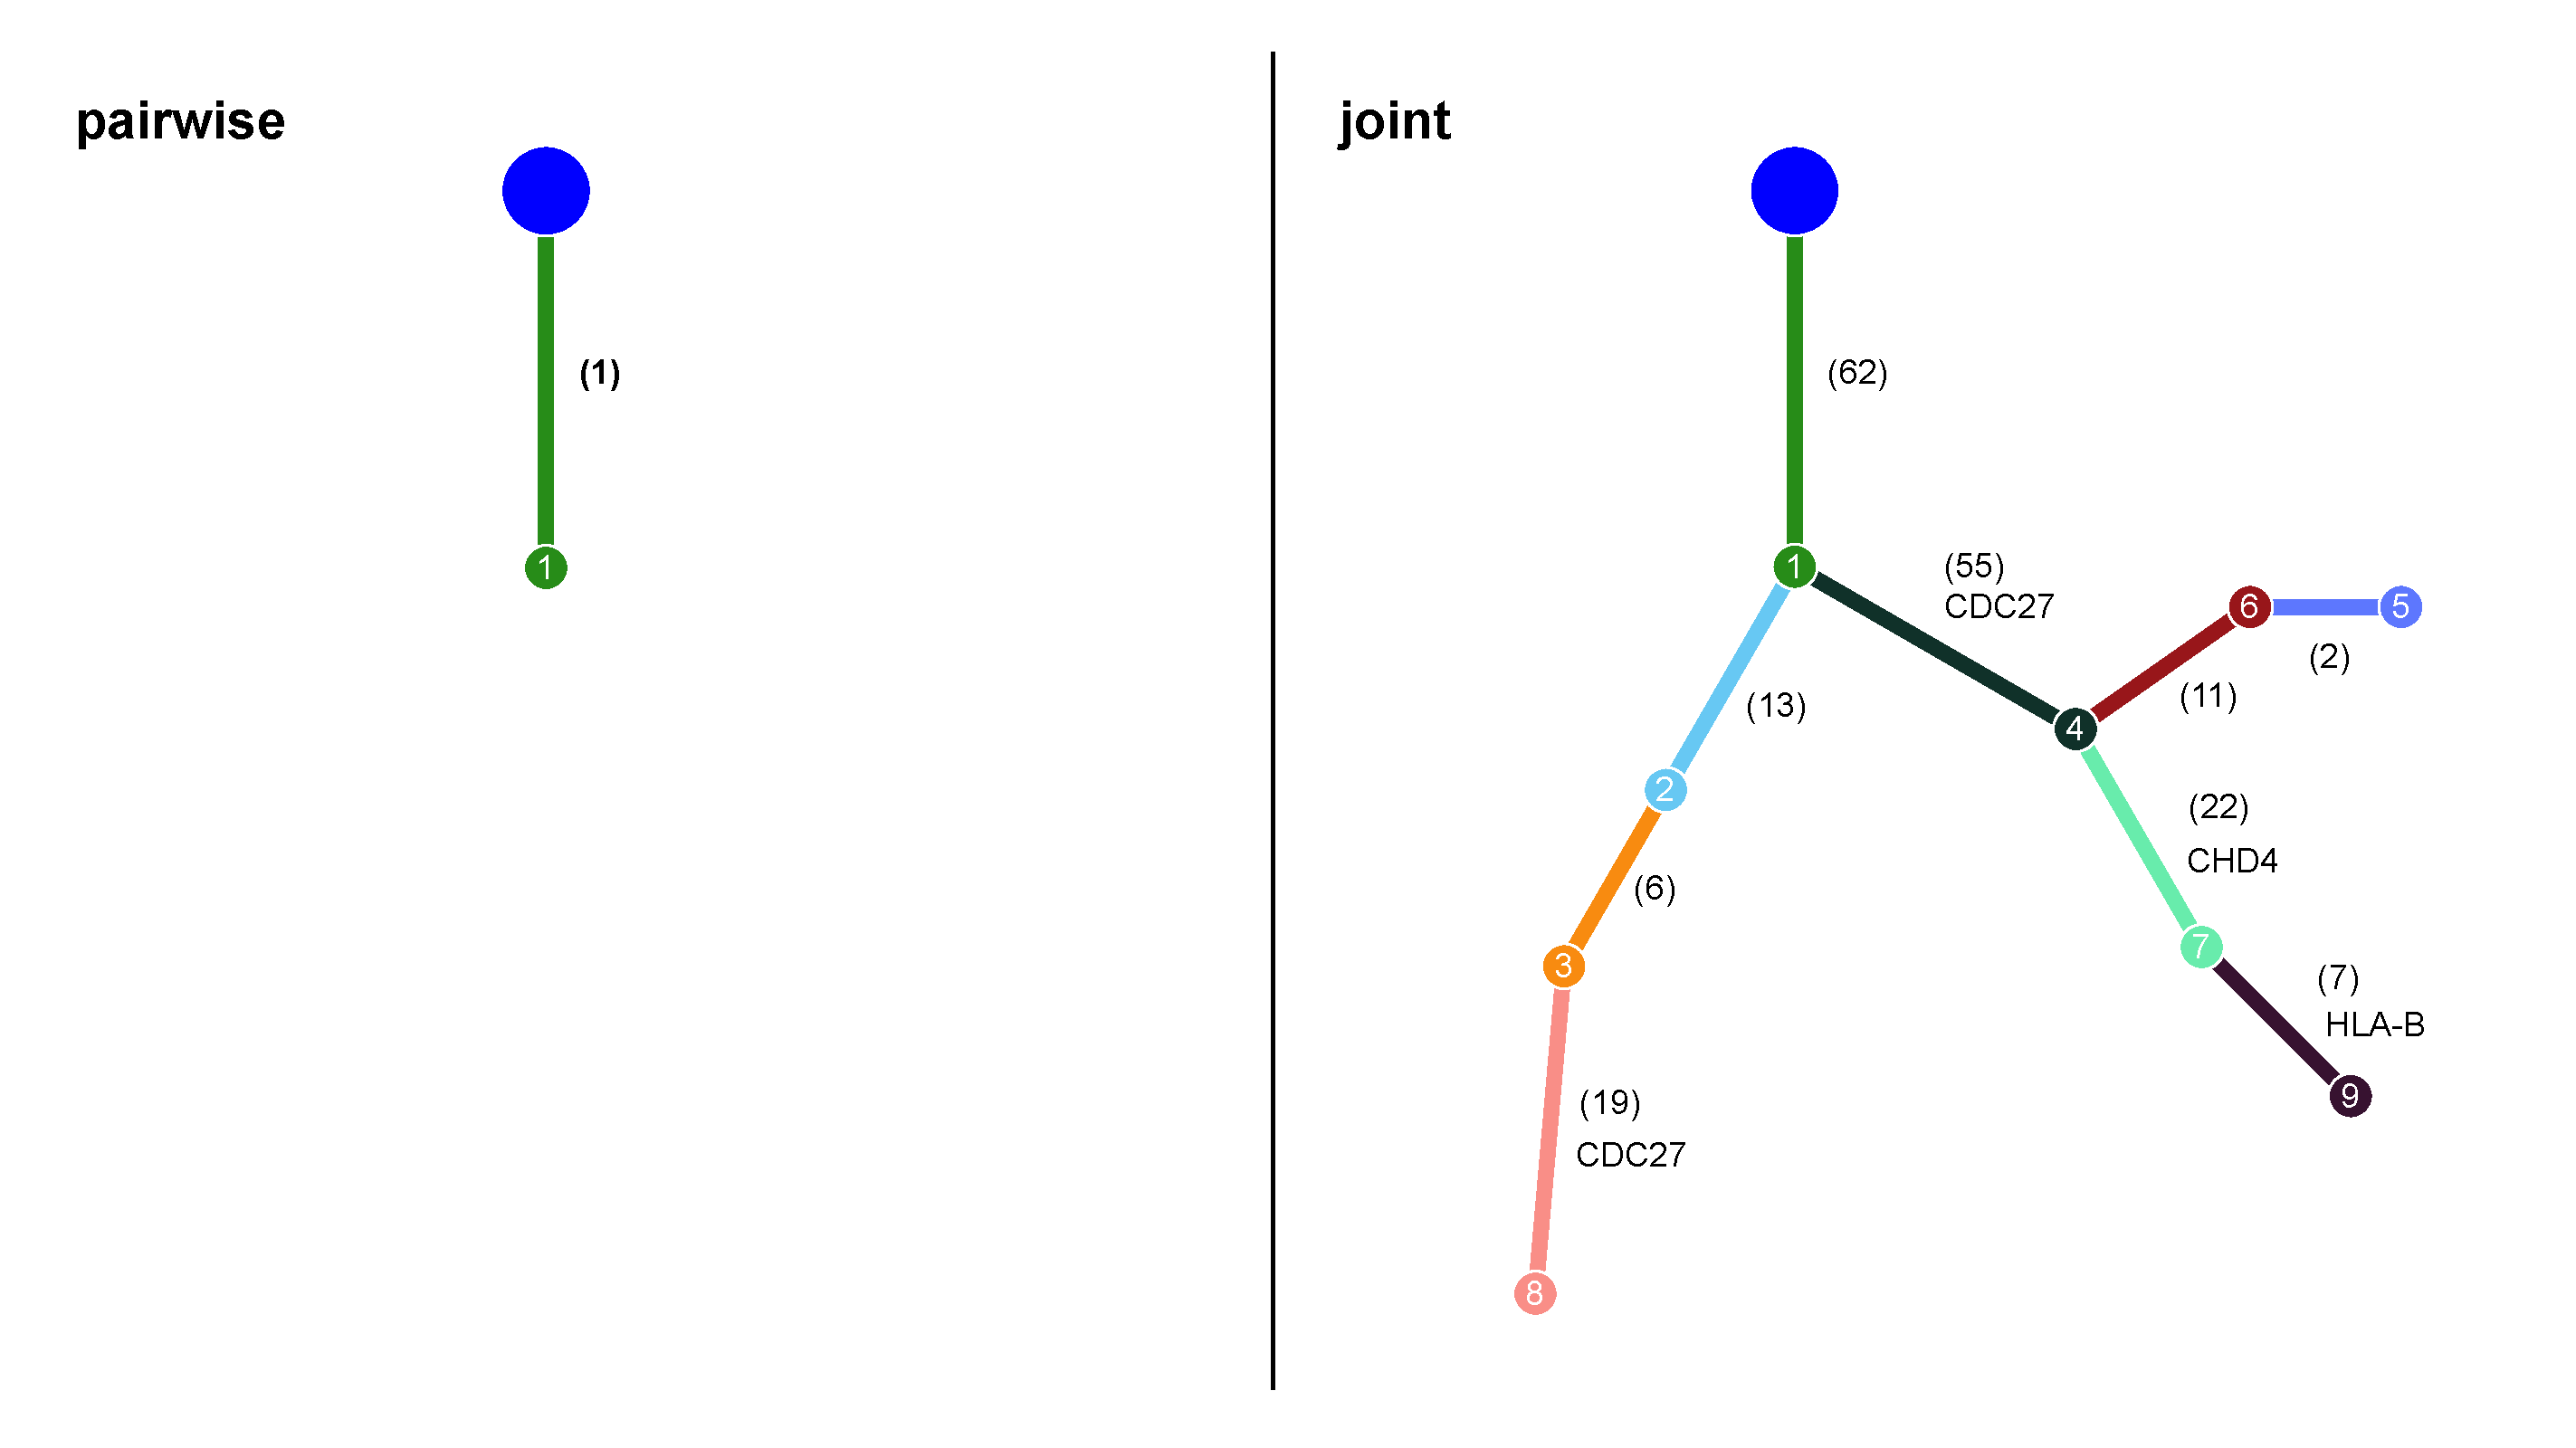
\includegraphics[width=.99\linewidth]{Figures/jointVariantCalling/clonalDeconv.pdf}
\caption[Reconstructed clonal trees for joint and pairwise variant calling]{Reconstructed clonal trees from PhylogicNDT; Blue circle at top depicts the germline/normal state. The coloured edges with the same coloured circle represents a distinct subclone of the parent from which the edge emerges; The number in braces next to the edge is the number of mutations which define this subclone with an added gene symbol added, if there is a cancer driver gene mutation. The left part shows the result when using the default pairwise method of Strelka2 and the right side uses the results from the Strelka2Pass workflow}\label{fig:clonaldeconv}
\end{figure}


\autoref{fig:clonaldeconv} shows the highest parsimony clonal tree reconstructed by PhylogicNDT for the pairwise as well as the joint variant calling. As the copynumber calling information is the same for both inputs, the only difference is in the called variants. While there was no subclonal structure detected at all for the pairwise analysis, there is a highly variable structure detected using the jointly called variants. As this is a clinical sample, we cannot be certaine that the more branched model is the actual truth, but its biologically more logical that a late stage cancer has developed several subclones, rather than it being a very homogeneous disease at all of the 10 sites at autopsy with no evolution over ten years of disease \cite{Gerstung2020}.
It is of particular interest, that the \textit{CDC27} gene got mutated at different time points in different clones (clone 8 vs. clone 4), which a clear sign of parallel evolution, which would definitely be missed without the joint analysis.


\subsection{Longitudinal enriched phylogeny}
\label{variantcalling-sec:fullphylo}
Of course it is finally also possible to build a phylogeny with the spatial tissue samples and the longitudinal ctDNA samples. However, as the ctDNA give a holistic view of all cancer metastases (\autoref{intro-sec:ctDNA}) the interpretation needs to accommodate for that. 

\begin{figure}[ht]
\centering
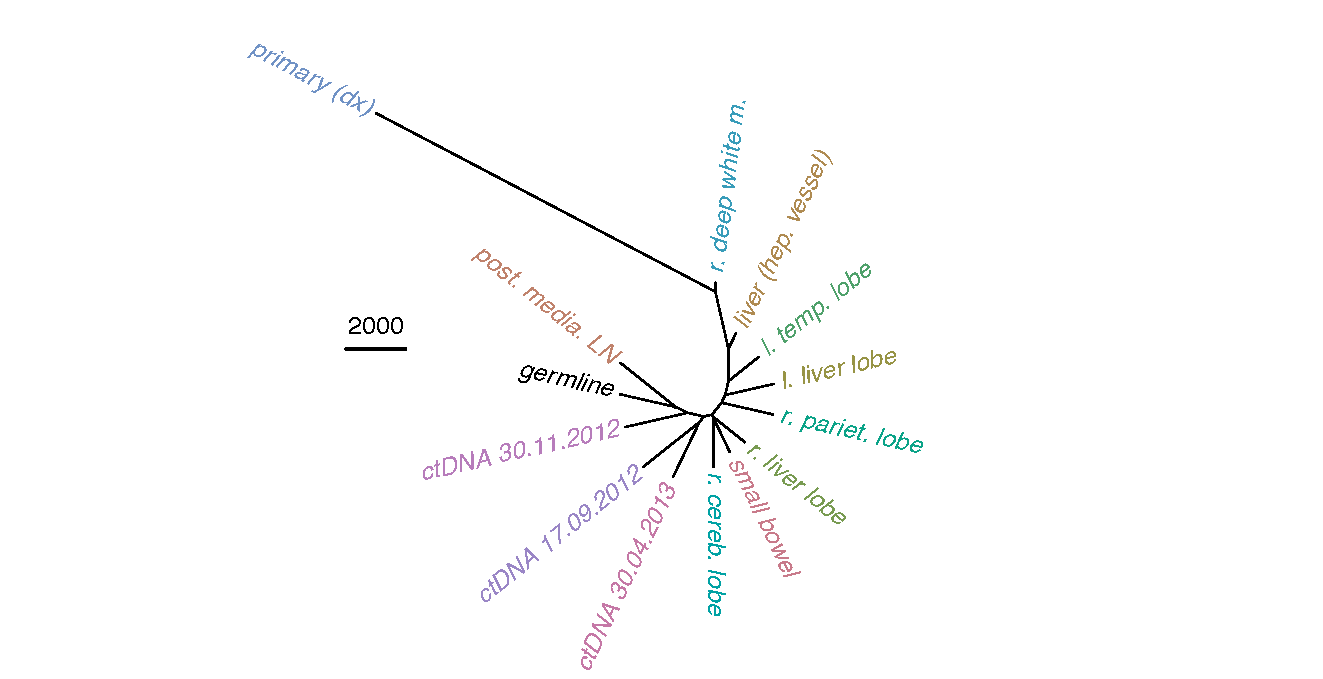
\includegraphics[width=.99\linewidth]{Figures/jointVariantCalling/phyloCA9_withctDNA.pdf}
\caption[Reconstructed phylogeny with longitudinal ctDNA samples]{Reconstructed phylogeny with longitudinal ctDNA samples: Tree from \autoref{fig:ca9phylo} with three additional ctDNA samples from different time points about one year prior to death. The ruler shows the equivalent of 2000 mutations} \label{fig:phyloCA9ctDNA}
\end{figure}

The maybe most surprising thing is that the more temporally distant ctDNA samples from 17.09.2012 and 30.04.2013 are in a subclade together, away from the ``ctDNA 30.11.2012`` sample. Secondly, the addition of the ctDNA samples also lead to a further bipartition edge, which separates ``r. liver lobe``, ``small bowel`` and ``r. cereb. lobe`` from the rest of the tree (\autoref{fig:phyloCA9ctDNA}). This was already inferable from the topology of the previous tree in \autoref{fig:tanglePhyloCA9} ``joint``, but is even more pronounced with the inclusion of the ctDNA samples.

This shows that the addition of more samples helps to refine and improve the trajectory and history of cancer samples and it is vital to do this analysis jointly to generate the optimal result.